\documentclass{ximera}

\newcommand{\RR}{\mathbb R}
\renewcommand{\d}{\,d}
\newcommand{\dd}[2][]{\frac{d #1}{d #2}}
\renewcommand{\l}{\ell}
\newcommand{\ddx}{\frac{d}{dx}}
\newcommand{\dfn}{\textbf}
\newcommand{\eval}[1]{\bigg[ #1 \bigg]}


\outcome{Identify word problems as related rates problems.}
\outcome{Solve related rates word problems.}
\outcome{Translate word problems into mathematical expressions.}

\title[Dig-In:]{Applied related rates}

\begin{document}
\begin{abstract}
  We solve related rates problems in context.
\end{abstract}
\maketitle

Now we are ready to solve related rates problems in context. Just as
before, we are going to follow essentially the same plan of attack in
each problem.


\begin{description}
\item[\textbf{Draw a picture.}] If possible, draw a schematic picture with all the relevant information. 
\item[\textbf{Find equations.}] We want equations that relate all
  relevant variables.
\item[\textbf{Differentiate.}] Here we will often use
  implicit differentiation.
\item[\textbf{Evaluate.}] Evaluate
  each quantity at the  relevant moment.
 \item[\textbf{Solve.}] Solve
 for the unknown rate at that moment.
\end{description}



\section{Formulas}


\begin{example}
A hand-tossed pizza crust starts off as a ball of dough with a volume
of $400\pi\, \text{cm}^3$. First, the cook stretches the dough to the
shape of a cylinder of radius $12$ cm. Next the cook tosses the
dough.

If during tossing, the dough maintains the shape of a cylinder and the
radius is increasing at a rate of $15$ cm/min, how fast is its
thickness changing when the radius is $20$ cm?
\begin{explanation}
  To start, \textbf{draw a picture}. Here we see a cylinder that
  represents our pizza dough.
  \begin{image}
  \begin{tikzpicture}
    \draw[penColor,very thick] (0,0) ellipse (2.5 and .8);
    \draw[very thick,penColor] (-2.5,-.5) arc (180:360:2.5 and .8);% bottom
    \draw[penColor] (0,0) -- (2.5,0);
    \draw[penColor,very thick] (-2.5,0) -- (-2.5,-.5);
    \draw[penColor,very thick] (2.5,0) -- (2.5,-.5);
    \node[above,penColor] at (1,0) {$r$};
    \node[below,penColor] at (1,0) {$r' = 15$};
    \draw[decoration={brace,raise=.2cm},decorate,thin] (2.5,0)--(2.5,-.5);
    \node [penColor,right] at (2.7,-.25) {$h$};
    \node [penColor,left] at (-1.5,1.2) {$V = 400\pi$ cm$^3$};
    \node [penColor, right] at (1.5,-1.42) {$V = \pi\cdot r^2 \cdot h$ cm$^3$};
  \end{tikzpicture}
  \end{image}
  Next we need to \textbf{find equations}. We see that we have
  \[
  400\pi = \answer[given]{\pi \cdot r^2 \cdot h},
  \]
  which immediately simplifies to
  \[
  400 = r^2 \cdot h.
  \]
  Since both $r$ and $h$ are functions of time, we now write
  \[
  400 = r(t)^2 \cdot h(t).
  \]
  Now we \textbf{differentiate} both sides of  the equation using implicit
  differentiation, treating all functions as functions of $t$,
  \[
  0 = 2\cdot r(t) \cdot r'(t) \cdot h(t) + r(t)^2 \cdot h'(t).
  \]
  Now we'll \textbf{evaluate} all  the quantities at the moment when $r=20$. 
  But, first, we have to compute $h$ at that moment. Since
  \[
 400 = 20^2 \cdot h, 
  \] it follows that $h=1$, when $r=20$. Now, we are ready.
  
 \[
 0 = 2\cdot 20 \cdot 15 \cdot 1 + 20^2 \cdot \Bigl[\frac{d}{dt}h\Bigr]_{r=20},
  \]
  \begin{align*}
    -2\cdot 20 \cdot 15  &= 20^2 \cdot  \Bigl[\frac{d}{dt}h\Bigr]_{r=20}\\
    \frac{-2\cdot 20 \cdot 15}{20^2}  &=  \Bigl[\frac{d}{dt}h\Bigr]_{r=20}\\
    -1.5  &=  \Bigl[\frac{d}{dt}h\Bigr]_{r=20}.
  \end{align*}
  Hence, the thickness of the dough is changing at a rate of $\answer[given]{-1.5}$
  cm/min.
\end{explanation}
\end{example}



\begin{example}
  Consider a melting snowball. We will assume that the rate at which the
  snowball is melting is proportional to its surface area. Show that
  the radius of the snowball is changing at a constant rate.
  
\begin{explanation}
  To start, \textbf{draw a picture}.
  \begin{image}
    \begin{tikzpicture}
      %\draw[penColor!50!background,very thick] (0,0) ellipse (2 and 1);
      \draw[very thick,penColor!20!background] (2,0) arc (0:180:2 and .7);% top half of ellipse
      \draw [penColor, very thick] (0,0) circle [radius=2];
      \draw[penColor] (0,0) -- (2,0);
      \node [below,penColor] at (1,0) {$r$ cm};
      \draw[very thick,penColor] (-2,0) arc (180:360:2 and .7);% bottom half of ellipse
      \node [penColor,left] at (-1.5,1.42) {$V = \frac{4}{3}\cdot \pi \cdot r^3$};
      \node [penColor, right] at (1.5,-1.42) {$A = 4\cdot \pi \cdot r^2$};
    \end{tikzpicture}
  \end{image}
  Next we need to \textbf{find equations}. The equations we'll use are
  \[
  V = \answer[given]{(4/3) \cdot \pi \cdot r^3} \qquad\text{and}\qquad A = \answer[given]{4\cdot
  \pi \cdot r^2}.
  \]
  Now the key words are ``the rate at which the snowball is melting is
  proportional to its surface area.'' From this we have the following
  equation:
  \begin{image}
    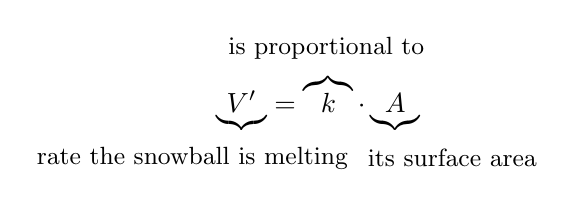
\begin{tikzpicture}
    \node at (0,0) {
      $\underbrace{V'} =  \overbrace{k} \cdot \underbrace{A}$
    };
    \node at (-1.6,-.7) {\small{rate the snowball is melting}};
    \node at (.1,.7) {\small{is proportional to}};
    \node at (1.7,-.7) {\small{its surface area}};
    \end{tikzpicture}
  \end{image}
  So we need to know $V'$. We know $V = \frac{4}{3}\cdot \pi\cdot
  r^3$. Since $r$ is a function of $t$, we  write 
    \[
  V(t) = \frac{4}{3}\cdot \pi\cdot r(t)^3.
  \]
So
  \[
  V'(t) = 4\cdot \pi\cdot r(t)^2 \cdot r'(t).
  \]
  We also know that
   \[
  V'(t) = k\cdot A(t).
  \]
  So,
  \[
 4\cdot \pi \cdot r(t)^2 \cdot r'(t) =  k\cdot 4\cdot
  \pi \cdot r(t)^2 .
  \]
 Therefore,
  \begin{align*}
r'(t) &=  k.\\
  \end{align*}
  Hence, the radius is changing at a constant rate. 
\end{explanation}
\end{example}

\section{Right triangles}

\begin{example}
A road running north to south crosses a road going east to west at the
point $P$.  Cyclist $A$ is riding north along the first road, and
cyclist $B$ is riding east along the second road.  At a particular
time, cyclist $A$ is $3$ kilometers to the north of $P$ and traveling
at $20$ km/hr, while cyclist $B$ is $4$ kilometers to the east of $P$
and traveling at $15$ km/hr.  How fast is the distance between the two
cyclists changing at that time?


\begin{explanation}
We start the same way we always do, we \textbf{draw a picture}.
\begin{image}
\begin{tikzpicture}
\draw[->,penColor!50!background, very thick] (-1,0) -- (4,0);
\draw[->,penColor!50!background, very thick] (0,-1) -- (0,4);
\draw[->,penColor, very thick] (0,3) -- (0,4);
\draw[->,penColor, very thick] (3,0) -- (4,0);
\draw [penColor, fill] (0,0) circle [radius=.07];
\draw [penColor, fill] (3,0) circle [radius=.07];
\draw [penColor, fill] (0,3) circle [radius=.07];
\draw[dashed,penColor2, very thick] (3,0) -- (0,3);

%\node[penColor,rotate=90,right] at (.5,3) {\scalebox{-2} \Bicycle};
\node[penColor,right] at (0,.2) {$P$};
\node[penColor,left] at (0,1.5) {$a(t)$ };
\node[penColor,left] at (-.005,3) {$A$ };
\node[penColor,below] at (1.5,0) {$b(t)$ };
\node[penColor,below] at (3,0) {B};
\node[penColor2,above] at (1.6,1.6) {$c(t)$};
%\node[penColor,right,above] at (3.5,0) {\scalebox{-2}[2] \Bicycle};
\end{tikzpicture}
\end{image}
Here $a(t)$ is the distance of cyclist $A$ north of $P$ at time $t$,
and $b(t)$ the distance of cyclist $B$ east of $P$ at time $t$, and
$c(t)$ is the distance from cyclist $A$ to cyclist $B$ at time $t$.

We must \textbf{find equations} relating variables $a$, $b$, and $c$.  By the Pythagorean Theorem,
\[
c(t)^2=a(t)^2+b(t)^2.
\] 
Now we can \textbf{differentiate} both sides of  the equation. 
\[
2c(t)c'(t)=2a(t)a'(t)+2b(t)b'(t).
\]
Now, let's draw and label the picture  at the time when $a=3$ and $b=4$.
\begin{image}
\begin{tikzpicture}
\draw[->,penColor!50!background, very thick] (-1,0) -- (4,0);
\draw[->,penColor!50!background, very thick] (0,-1) -- (0,4);
\draw[->,penColor, very thick] (0,3) -- (0,4);
\draw[->,penColor, very thick] (3,0) -- (4,0);
\draw [penColor, fill] (0,0) circle [radius=.07];
\draw [penColor, fill] (3,0) circle [radius=.07];
\draw [penColor, fill] (0,3) circle [radius=.07];
\draw[dashed,penColor2, very thick] (3,0) -- (0,3);

%\node[penColor,rotate=90,right] at (.5,3) {\scalebox{-2} \Bicycle};
\node[penColor,right] at (0,.2) {$P$};
\node[penColor,left] at (-.005,3) {$\frac{da}{dt} = 20$ km/hr A};
\node[penColor,left] at (0,1.5) {$3$ km};
\node[penColor,below] at (1.5,0) {$4$ km};
\node[penColor,below] at (4,0) {B  $\frac{db}{dt}= 15$ km/hr };
\node[penColor2,above] at (1.6,1.6) {$c$};
%\node[penColor,right,above] at (3.5,0) {\scalebox{-2}[2] \Bicycle};
\end{tikzpicture}
\end{image}
 We have to find the distance $c$ at that time.
By the the Pythagorean Theorem and the picture above, it follows that
\[
c = \answer[given]{5}  km
\]
Now we  \textbf{evaluate} all the quantities at the time when $a=3$ and $b=4$, and get 
\[
2\cdot 5 \cdot \Bigl[\frac{dc}{dt}\Bigr]_{a=3, b=4} = 2 \cdot 3\cdot 20 + 2 \cdot 4 \cdot 15.
\]
Solving for $\Bigl[\frac{dc}{dt}\Bigr]_{a=3, b=4}$ we find\\

 $\Bigl[\frac{dc}{dt}\Bigr]_{a=3, b=4} = \answer[given]{24}$ km/hr.
\end{explanation}
\end{example}


\begin{example}
A plane is flying at an altitude of $3$ miles directly away from you at $500$ mph 
.  How fast is the plane's distance from you increasing at
the moment when the plane is flying over a point on the ground $4$
miles from you?


\begin{explanation}
To start, \textbf{draw a picture}.
\begin{image}
\begin{tikzpicture}
\draw[penColor2, dashed, very thick] (0,0) -- (5,4);
%\draw[penColor, dashed, very thick] (0,0) -- (0,4);
\draw[penColor, dashed, very thick] (0,0) -- (0,4);
\draw[penColor, dashed, very thick] (0,0) -- (5,0);
\draw[->,penColor, very thick] (0,4) -- (6,4);
\draw [penColor, fill] (5,4) circle [radius=.07];
%\node [left,penColor] at (0,0) {\scalebox{3} \Ladiesroom};
%\node [right,penColor] at (6,4) {\scalebox{3}{\ding{40}}};
\node [right,penColor] at (0,2) {$3$ miles};
\node [above,penColor] at (2.6,4) {$p(t)$ };
\node [above,penColor] at (5,4) {$plane$ };
\node [above,penColor] at (2.6,3.1) {$\frac{dp}{dt}=500$mph};
\node [below,penColor] at (2.5,0) {ground};
\node [left,penColor2] at (3.3,2) {$s(t)$ };
\draw [penColor, fill] (0,0) circle [radius=.07];
\node [left,penColor] at (-.1,0) {You};
\end{tikzpicture}
\end{image}
Next we need to \textbf{find equations}. By the Pythagorean Theorem
we know that
\[
p^2+3^2=s^2.
\] 
Since  $p$ and $s$ are functions of time, we now
\textbf{differentiate} both sides of the equation. We write
\[
2\cdot p(t)\cdot p'(t)  = 2\cdot s(t) \cdot s'(t).
\] 
Now, let's draw and  the picture at the moment when $p=4$ mi.
\begin{image}
\begin{tikzpicture}
\draw[penColor2, dashed, very thick] (0,0) -- (5,4);
\draw[penColor2, dashed, very thick] (5,0) -- (5,4);
%\draw[penColor, dashed, very thick] (0,0) -- (0,4);
\draw[penColor, dashed, very thick] (0,0) -- (0,4);
\draw[penColor, dashed, very thick] (0,0) -- (5,0);
\draw[->,penColor, very thick] (0,4) -- (6,4);
\draw [penColor, fill] (5,4) circle [radius=.07];
\draw [penColor, fill] (5,0) circle [radius=.07];
%\node [left,penColor] at (0,0) {\scalebox{3} \Ladiesroom};
%\node [right,penColor] at (6,4) {\scalebox{3}{\ding{40}}};
\node [right,penColor] at (0,2) {$3$ miles};
\node [right,penColor] at (5,2) {$3$ miles};
\node [right,penColor] at (5,0.25) {point on the ground};
\node [right,penColor] at (5,0) {4 miles away from you };
\node [above,penColor] at (2.6,3.1) {$\frac{dp}{dt} = 500$ mph};
\node [above,penColor] at (2.6,4) {$p=4$ miles};
\node [above,penColor] at (5,4) {$plane$ };
\node [below,penColor] at (2.5,0) {$4$ miles};
\node [left,penColor2] at (3.5,2) {$s=5$ };
\draw [penColor, fill] (0,0) circle [radius=.07];
\node [left,penColor] at (-.1,0) {You};
\end{tikzpicture}
\end{image}
Now we'll \textbf{evaluate} all the quantities at the moment when $p=4$ miles. 
Additionally, at this time we know that $4^2+3^2=s^2$, so
$s=\answer[given]{5}$.  Putting together all the information we get
\[
2(4)(500)=2(5)\Bigl[\frac{ds}{dt}\Bigr]_{p=4} .
\]
Finally, we solve for $\Bigl[\frac{ds}{dt}\Bigr]_{p=4}$.\\

$\Bigl[\frac{ds}{dt}\Bigr]_{p=4}=\answer[given]{400}$ mph.
\end{explanation}
\end{example}


\section{Angular rates}

\author{Nela Lakos}
\begin{example}
A plane is flying at an altitude of $3$ miles directly away from you at $500$ mph 
.  Let  $\theta$ be the \textbf{angle of elevation} of the plane, i.e., the angle between the ground and  line of  your sight to the plane.
How fast is the angle $\theta$  decreasing at
the moment when the plane is flying over a point on the ground $4$
miles from you?


\begin{explanation}
  First, note that the unknown rate of change, $\Bigl [\frac{d\theta}{dt}\Bigr]_{p=4}$, should be measured in rad/s.
  Therefore, we have to convert the units of the given rate of change, mph, into mi/s:
    $\frac{dp}{dt}=500$mph$=\frac{500}{60\cdot60}$ mi/s. \\
Next, we \textbf{draw a picture}.
\begin{image}
\begin{tikzpicture}
\draw[penColor2, dashed, very thick] (0,0) -- (5,4);
%\draw[penColor, dashed, very thick] (0,0) -- (0,4);
\draw[penColor, dashed, very thick] (0,0) -- (0,4);
\draw[penColor, dashed, very thick] (5,0) -- (5,4);
\draw[penColor, dashed, very thick] (0,0) -- (5,0);
\draw[->,penColor, very thick] (0,4) -- (6,4);
\draw [penColor, fill] (5,4) circle [radius=.07];
\coordinate (A) at (3.3,2.6);
        \coordinate (B) at (0,0);
        \coordinate (C) at (4,0);
\tkzMarkAngle[size=2cm,thin](C,B,A)
        \tkzLabelAngle[pos = 1.3](C,B,A){$\theta$}
%\node [left,penColor] at (0,0) {\scalebox{3} \Ladiesroom};
%\node [right,penColor] at (6,4) {\scalebox{3}{\ding{40}}};
\node [right,penColor] at (5,2) {$3$ miles};
\node [above,penColor] at (2.6,4) {$p(t)$ };
\node [above,penColor] at (5,4) {$plane$ };
\node [above,penColor] at (2.18,3.1) {$\frac{dp}{dt}=\frac{500}{60\cdot60}$mi/s};
\node [below,penColor] at (2.5,0) {ground};
\draw [penColor, fill] (0,0) circle [radius=.07];
\node [left,penColor] at (-.1,0) {You};
\end{tikzpicture}
\end{image}
Now we need to \textbf{find an equation} relating variables $p$ and $\theta$.
From the picture we can see that
\[
\tan{\theta}=\frac{3}{p}.
\] 
Since  $p$ and $\theta$ are functions of time, we now
\textbf{differentiate} both sides of the equation. We write
\[
\sec^{2}{\theta}\cdot\theta'  = -\frac{3}{p^2}\cdot p'.
\] 
Now, we draw and label the picture at the moment when $p=4$ mi.
\begin{image}
\begin{tikzpicture}
\draw[penColor2, dashed, very thick] (0,0) -- (5,4);
\draw[penColor2, dashed, very thick] (5,0) -- (5,4);
%\draw[penColor, dashed, very thick] (0,0) -- (0,4);
\draw[penColor, dashed, very thick] (0,0) -- (0,4);
\draw[penColor, dashed, very thick] (0,0) -- (5,0);
\draw[->,penColor, very thick] (0,4) -- (6,4);
\draw [penColor, fill] (5,4) circle [radius=.07];
\draw [penColor, fill] (5,0) circle [radius=.07];
\coordinate (A) at (3.3,2.6);
        \coordinate (B) at (0,0);
        \coordinate (C) at (4,0);
\tkzMarkAngle[size=2cm,thin](C,B,A)
        \tkzLabelAngle[pos = 1.3](C,B,A){$\theta$}
%\node [left,penColor] at (0,0) {\scalebox{3} \Ladiesroom};
%\node [right,penColor] at (6,4) {\scalebox{3}{\ding{40}}};
\node [right,penColor] at (0,2) {$3$ miles};
\node [right,penColor] at (5,2) {$3$ miles};
\node [right,penColor] at (5,0.25) {point on the ground};
\node [right,penColor] at (5,0) {4 miles away from you };
\node [above,penColor] at (2.6,3.1) {$\frac{dp}{dt} =\frac{500}{60\cdot60}$mi/s};
\node [above,penColor] at (2.6,4) {$p=4$ miles};
\node [above,penColor] at (5,4) {$plane$ };
\node [below,penColor] at (2.5,0) {$4$ miles};
\draw [penColor, fill] (0,0) circle [radius=.07];
\node [left,penColor] at (-.1,0) {You};
\end{tikzpicture}
\end{image}

We will now evaluate all the quantities at the moment when $p=4$. First, we have to compute $\sec^{2}{\theta}$ at that time.
We will remind ourselves of the trig identity
\[
\sec^2{\theta}=1+\tan^2{\theta}.
\] 
So,
\[
\Big[\sec^2{\theta}\Bigr]_{p=4}=1+\Bigr(\frac{3}{4}\Bigl)^2=\frac{25}{16}.
\] 
Now, by substituting all the known values into the equation above, we get
\[
\frac{25}{16}\cdot\Bigl [\frac{d\theta}{dt}\Bigr]_{p=4} = -\frac{3}{16}\cdot \frac{500}{60\cdot60}.
\] 
Now we solve for $\Bigl [\frac{d\theta}{dt}\Bigr]_{p=4}$ and get that
\[
\Bigl [\frac{d\theta}{dt}\Bigr]_{p=4} = -\frac{1}{60}  rad/s.
\] 
\end{explanation}
\end{example}

\section{Similar triangles}

\begin{example}
  It is night. Someone who is $6$ feet tall is walking away from a
  street light at a rate of $3$ feet per second.  The street light is
  $15$ feet tall.  The person casts a shadow on the ground in front of
  them. How fast is the length of the shadow growing when the person
  is $7$ feet from the street light?

  \begin{explanation}
    To start, \textbf{draw a picture}.
    \begin{image}
      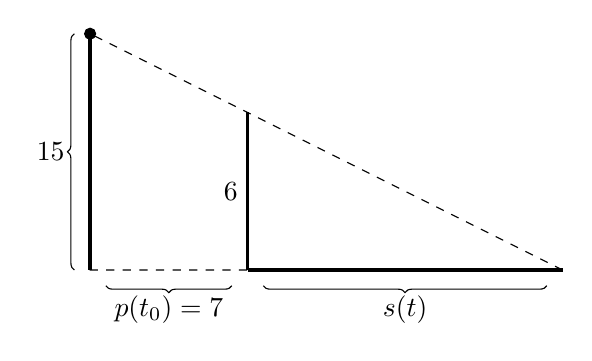
\begin{tikzpicture}
        \coordinate (A) at (6,2);
        \coordinate (B) at (0,5);
        \coordinate (C) at (0,2);
        \coordinate (D) at (2,2);
        \coordinate (E) at (2,4);
        \tkzMarkRightAngle(A,C,B)
        \tkzMarkRightAngle(A,D,E)
        \tkzDefMidPoint(A,B) \tkzGetPoint{a}
        \tkzDefMidPoint(A,C) \tkzGetPoint{b}
        \tkzDefMidPoint(D,C) \tkzGetPoint{x}
        \draw[decoration={brace,mirror,raise=.2cm},decorate,thin] (.2,2)--(1.8,2);
        \draw[decoration={brace,mirror,raise=.2cm},decorate,thin] (2.2,2)--(5.8,2);
        \draw[decoration={brace,raise=.2cm},decorate,thin] (0,2)--(0,5);
        \draw[dashed] (A)--(B)--(C)--cycle;
        \draw[very thick] (D)--(E);
        \draw[very thick] (D)--(A);
        \draw[very thick] (B)--(C);
        \node[left] at (2,3) {$6$};
        \node at (1,2-.5) {$p(t_0)=7$};
        \node at (4,2-.5) {$s(t)$};
        \node at (0-.5,3.5) {$15$};
        \draw [fill] (0,5) circle [radius=.07];
      \end{tikzpicture}
    \end{image}
    Here $t$ is the variable and $t_0$ is the specific time when
    $p(t_0) = 7$.
    
    Now we need to \textbf{find equations}. We use the fact that we
    have similar triangles to write:
    \begin{align*}
      \frac{s(t)+p(t)}{\answer[given]{15}} &= \frac{s(t)}{\answer[given]{6}},\\
      6\cdot s(t) + 6 \cdot p(t) &= 15\cdot s(t),\\
      6\cdot p(t) &=9\cdot s(t),\\
      2\cdot p(t) &=3 \cdot s(t). \\
    \end{align*}
    Now we must \textbf{differentiate the equation}. We should use
    implicit differentiation, and treat each of the variables as
    functions of $t$. Write
    \[
    2\cdot p'(t) =3 \cdot s'(t)
    \]
    At this point we \textbf{evaluate and solve}. Since the person is waling at a rate of $3$ feet per second, we may write
    \[
    2\cdot 3 = 3 \cdot s'(t),
    \]
    and cancel to see that $s'(t) = \answer[given]{2}$, meaning the shadow is growing
    at a rate of $2$ feet per second.
  \end{explanation}
\end{example}
\begin{example}
Water is poured into a conical container at the rate of 10
cm${}^3$/sec.  The cone points directly down, and it has a height of
30 cm and a base radius of 10 cm.  How fast is the water level rising
when the water is 4 cm deep?

\begin{explanation}
To start, \textbf{draw a picture}.
\begin{image}
\begin{tikzpicture}
\draw[penColor,very thick] (0,4) ellipse (4 and 1);
\draw[very thick,penColor!20!background] (2,2) arc (0:180:2 and .5);% top half of ellipse
\draw[very thick,penColor] (-2,2) arc (180:360:2 and .5);% bottom half of ellipse
\draw[penColor, very thick] (3.97,3.85) -- (0,0);
\draw[penColor, very thick] (-3.97,3.85) -- (0,0);
\draw[penColor, very thick] (0,4) -- (4,4);
\draw[penColor!50!background, very thick] (0,2) -- (2,2);
\draw[->,line width=0.4cm, penColor!20!background] (0,6) -- (0,4.25);
\draw[dashed, penColor2, very thick] (2.1,0) -- (2.1,2);
\draw[dashed, penColor, very thick] (-4.1,0) -- (-4.1,4);
\node[right, penColor] at (.4,5.6) {$\dd[V]{t} = 10$ cm$^3$/sec};
\node[below, penColor] at (2,4) {$10$ cm};
\node[above, penColor] at (1,2) {$r$ cm};
\node[right, penColor2] at (2.1,1) {$h(t) = 4$ cm};
\node[left, penColor] at (-4.1,2) {$30$ cm};
\end{tikzpicture}
\end{image}
Note, no attempt was made to draw this picture to scale, rather we
want all of the relevant information to be available to the
mathematician.

Now we need to \textbf{find equations}. The formula for the volume of
a cone tells us that
\[
V = \frac{\pi}{3} r^2 h.
\]
Also the dimensions of the cone of water must have the same
proportions as those of the container.  That is, because of similar
triangles,
\[
\frac{r}{h}=\frac{10}{30} \qquad\text{so}\qquad r=\answer[given]{h/3}.
\]  
Now we must \textbf{differentiate the equation}. We should use
implicit differentiation, and treat each of the variables as functions
of $t$. Write
\[
\dd[V]{t} = \frac{\pi}{3}\left(2rh \dd[r]{t} + r^2 \dd[h]{t}\right)
\qquad\text{and}\qquad \dd[r]{t} = \frac{1}{3}\cdot \dd[h]{t}.
\]
At this point we \textbf{evaluate and solve}. We plug in $\dd[V]{t} =
\answer[given]{10}$, $r = \answer[given]{4/3}$, $\dd[r]{t} = \frac{1}{3}\cdot \dd[h]{t}$ and
$h=\answer[given]{4}$. Write
\begin{align*}
10 &= \frac{\pi}{3}\left(2\cdot \frac{4}{3}\cdot 4 \cdot\frac{1}{3}\cdot\dd[h]{t} + \left(\frac{4}{3}\right)^2 \dd[h]{t}\right)\\
10 &= \frac{\pi}{3}\left(\frac{32}{9}\dd[h]{t} + \frac{16}{9} \dd[h]{t}\right)\\
10 &= \frac{16\pi}{9}\dd[h]{t}\\
\frac{90}{16\pi} &= \dd[h]{t}.
\end{align*}
Thus, $\dd[h]{t}=\answer[given]{\frac{90}{16\pi}}$ cm/sec.
\end{explanation}
\end{example}
\end{document}



